    \hypertarget{notebooks-jupyter-comme-support-de-cours}{%
\section{``Notebooks'' Jupyter comme support de
cours}\label{notebooks-jupyter-comme-support-de-cours}}

    Pour illustrer les vidéos du MOOC, nous avons choisi d'utiliser Jupyter
pour vous rédiger les documents ``mixtes'' contenant du texte et du code
Python, qu'on appelle des ``notebooks'', et dont le présent document est
un exemple.

Nous allons, dans la suite, utiliser du code Python, pourtant nous
n'avons pas encore abordé le langage. Pas d'inquiétude, ce code est
uniquement destiné à valider le fonctionnement des notebooks, et nous
n'utilisons que des choses très simples.

    \hypertarget{avertissement-ruxe9glages-du-navigateur}{%
\subsubsection{Avertissement: réglages du
navigateur}\label{avertissement-ruxe9glages-du-navigateur}}

    Avant toute chose, pour un bon fonctionnement des notebooks, on rappelle
qu'il est nécessaire d'avoir \textbf{autorisé} dans votre navigateur les
\textbf{cookies} en provenance du site Internet
\textbf{\texttt{nbhosting.inria.fr}}, qui héberge l'infrastructure qui
héberge tous les notebooks.

    \hypertarget{avantages-des-notebooks}{%
\subsubsection{Avantages des notebooks}\label{avantages-des-notebooks}}

    Comme vous le voyez, ce support permet un format plus lisible que des
commentaires dans un fichier de code.

    Nous attirons votre attention sur le fait que \textbf{les fragments de
code peuvent être évalués et modifiés}. Ainsi vous pouvez facilement
essayer des variantes autour du notebook original.

Notez bien également que le code Python est interprété \textbf{sur une
machine distante}, ce qui vous permet de faire vos premiers pas avant
même d'avoir procédé à l'installation de Python sur votre propre
ordinateur.

    \hypertarget{comment-utiliser-les-notebooks}{%
\subsubsection{Comment utiliser les
notebooks}\label{comment-utiliser-les-notebooks}}

    En haut du notebook, vous avez une barre de menu (sur fond bleu clair),
contenant~:

\begin{itemize}
	\item
un titre pour le notebook, avec un numéro de version~;
	\item
une barre de menus avec les entrées \texttt{File}, \texttt{Insert},
\texttt{Cell}, \texttt{Kernel};
	\item
et une barre de boutons qui sont des
raccourcis vers certains menus fréquemment utilisés. Si vous laissez
votre souris au dessus d'un bouton, un petit texte apparaît, indiquant à
quelle fonction correspond ce bouton.
\end{itemize}

Nous avons vu dans la vidéo qu'un notebook est constitué d'une suite de
cellules, soit textuelles, soit contenant du code. Les cellules de code
sont facilement reconnaissables, elles sont précédées de
\texttt{In\ {[}\ {]}:}. La cellule qui suit celle que vous êtes en train
de lire est une cellule de code.

Pour commencer, sélectionnez cette cellule de code avec votre souris, et
appuyez dans la barre de menu - en haut du notebook, donc - sur celui en
forme de flèche triangulaire vers la droite (Play)~: 

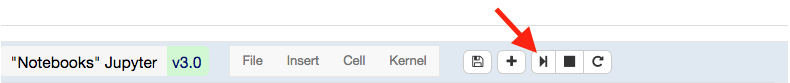
\includegraphics{medias/notebook-eval-button.png}\\
    \begin{Verbatim}[commandchars=\\\{\}]
{\color{incolor}In [{\color{incolor}1}]:} \PY{l+m+mi}{20} \PY{o}{*} \PY{l+m+mi}{30}
\end{Verbatim}


\begin{Verbatim}[commandchars=\\\{\}]
{\color{outcolor}Out[{\color{outcolor}1}]:} 600
\end{Verbatim}
            
    Comme vous le voyez, la cellule est ``exécutée'' (on dira plus
volontiers évaluée), et on passe à la cellule suivante.

Alternativement, vous pouvez simplement taper au clavier
\textbf{\emph{Shift+Enter}}, ou selon les claviers
\textbf{\emph{Maj-Entrée}}, pour obtenir le même effet. D'une manière
générale, il est important d'apprendre et d'utiliser les raccourcis
clavier, cela vous fera gagner beaucoup de temps par la suite.

    La façon habituelle d'\emph{exécuter} l'ensemble du notebook consiste~:
\begin{itemize}
	\item
	à sélectionner la première cellule,
	\item
	et à taper \textbf{\emph{Shift+Enter}} jusqu'à attendre la fin du notebook.
\end{itemize}

    Lorsqu'une cellule de code a été évaluée, Jupyter ajoute sous la cellule
\texttt{In} une cellule \texttt{Out} qui donne le résultat du fragment
Python, soit ci-dessus 600.\\

Jupyter ajoute également un nombre entre les crochets pour afficher, par
exemple ci-dessus, \texttt{In\ {[}1{]}:}. Ce nombre vous permet de
retrouver l'ordre dans lequel les cellules ont été évaluées.

    Vous pouvez naturellement modifier ces cellules de code pour faire des
essais~; ainsi vous pouvez vous servir du modèle ci-dessous pour
calculer la racine carrée de 3, ou essayer la fonction sur un nombre
négatif et voir comment est signalée l'erreur.

    \begin{Verbatim}[commandchars=\\\{\}]
{\color{incolor}In [{\color{incolor}2}]:} \PY{c+c1}{\PYZsh{} math.sqrt (pour square root) calcule la racine carrée}
        \PY{k+kn}{import} \PY{n+nn}{math}
        \PY{n}{math}\PY{o}{.}\PY{n}{sqrt}\PY{p}{(}\PY{l+m+mi}{2}\PY{p}{)}
\end{Verbatim}


\begin{Verbatim}[commandchars=\\\{\}]
{\color{outcolor}Out[{\color{outcolor}2}]:} 1.4142135623730951
\end{Verbatim}
            
    On peut également évaluer tout le notebook en une seule fois en
utilisant le menu \emph{Cell -\textgreater{} Run All}.

    \hypertarget{attention-uxe0-bien-uxe9valuer-les-cellules-dans-lordre}{%
\subsubsection{Attention à bien évaluer les cellules dans
l'ordre}\label{attention-uxe0-bien-uxe9valuer-les-cellules-dans-lordre}}

    Il est important que les cellules de code soient évaluées dans le bon
ordre. Si vous ne respectez pas l'ordre dans lequel les cellules de code
sont présentées, le résultat peut être inattendu.\\

En fait, évaluer un programme sous forme de notebook revient à le
découper en petits fragments, et si on exécute ces fragments dans le
désordre, on obtient naturellement un programme différent.

    On le voit sur cet exemple~:

    \begin{Verbatim}[commandchars=\\\{\}]
{\color{incolor}In [{\color{incolor}3}]:} \PY{n}{message} \PY{o}{=} \PY{l+s+s2}{\PYZdq{}}\PY{l+s+s2}{Il faut faire attention à l}\PY{l+s+s2}{\PYZsq{}}\PY{l+s+s2}{ordre dans lequel on évalue les notebooks}\PY{l+s+s2}{\PYZdq{}}
\end{Verbatim}


    \begin{Verbatim}[commandchars=\\\{\}]
{\color{incolor}In [{\color{incolor}4}]:} \PY{n+nb}{print}\PY{p}{(}\PY{n}{message}\PY{p}{)}
\end{Verbatim}


    \begin{Verbatim}[commandchars=\\\{\}]
Il faut faire attention à l'ordre dans lequel on évalue les notebooks

    \end{Verbatim}

    Si un peu plus loin dans le notebook on fait par exemple~:

    \begin{Verbatim}[commandchars=\\\{\}]
{\color{incolor}In [{\color{incolor}5}]:} \PY{c+c1}{\PYZsh{} ceci a pour effet d\PYZsq{}effacer la variable \PYZsq{}message\PYZsq{}}
        \PY{k}{del} \PY{n}{message}
\end{Verbatim}


    qui rend le symbole \texttt{message} indéfini, alors bien sûr on ne peut
plus évaluer la cellule qui fait \texttt{print} puisque la variable
\texttt{message} n'est plus connue de l'interpréteur.

    \hypertarget{ruxe9initialiser-linterpruxe9teur}{%
\subsubsection{Réinitialiser
l'interpréteur}\label{ruxe9initialiser-linterpruxe9teur}}

    Si vous faites trop de modifications, ou perdez le fil de ce que vous
avez évalué, il peut être utile de redémarrer votre interpréteur. Le
menu \emph{Kernel~→~Restart} vous permet de faire cela, un peu à la
manière de IDLE qui repart d'un interpréteur vierge lorsque vous
utilisez la fonction F5.

    Le menu \emph{Kernel~→~Interrupt} peut être quant à lui utilisé si votre
fragment prend trop longtemps à s'exécuter (par exemple vous avez écrit
une boucle dont la logique est cassée et qui ne termine pas).

    \hypertarget{vous-travaillez-sur-une-copie}{%
\subsubsection{Vous travaillez sur une
copie}\label{vous-travaillez-sur-une-copie}}

    Un des avantages principaux des notebooks est de vous permettre de
modifier le code que nous avons écrit, et de voir par vous-mêmes comment
se comporte le code modifié.\\

Pour cette raison, chaque élève dispose de sa \textbf{propre copie} de
chaque notebook, vous pouvez bien sûr apporter toutes les modifications
que vous souhaitez à vos notebooks sans affecter les autres étudiants.

    \hypertarget{revenir-uxe0-la-version-du-cours}{%
\subsubsection{Revenir à la version du
cours}\label{revenir-uxe0-la-version-du-cours}}

    Vous pouvez toujours revenir à la version ``du cours'' grâce au menu
\emph{File~→~Reset to original}.\\

    Attention, avec cette fonction vous restaurez \textbf{tout le notebook}
et donc \textbf{vous perdez vos modifications sur ce notebook}.

    \hypertarget{tuxe9luxe9charger-au-format-python}{%
\subsubsection{Télécharger au format
Python}\label{tuxe9luxe9charger-au-format-python}}

    Vous pouvez télécharger un notebook au format Python sur votre
ordinateur grâce au menu \emph{File~→~Download~as~→~Python}

    Les cellules de texte sont préservées dans le résultat sous forme de
commentaires Python.

    \hypertarget{partager-un-notebook-en-lecture-seule}{%
\subsubsection{Partager un notebook en lecture
seule}\label{partager-un-notebook-en-lecture-seule}}

    Enfin, avec le menu \emph{File~→~Share~static~version}, vous pouvez
publier une version en lecture seule de votre notebook~; vous obtenez
une URL que vous pouvez publier, par exemple pour demander de l'aide sur
le forum. Ainsi, les autres étudiants peuvent accéder en lecture seule à
votre code.\\

    Notez que lorsque vous utilisez cette fonction plusieurs fois, c'est
toujours la dernière version publiée que verront vos camarades, l'URL
utilisée reste toujours la même pour un étudiant et un notebook donné.

    \hypertarget{ajouter-des-cellules}{%
\subsubsection{Ajouter des cellules}\label{ajouter-des-cellules}}

    Vous pouvez ajouter une cellule n'importe où dans le document avec le
bouton \textbf{+} de la barre de boutons.\\

Aussi, lorsque vous arrivez à la fin du document, une nouvelle cellule
est créée chaque fois que vous évaluez la dernière cellule~; de cette
façon vous disposez d'un brouillon pour vos propres essais.\\

À vous de jouer.
